% !TEX root = ../YourName-Dissertation.tex

\chapter{Questions on the  local level}
This chapter talks about the reaction of subnational governments in the interaction with central government.The most frequently investigated question is the effect of IGT, A bunch of scholars devote time and energy to analyze and evaluate the impact of intergovernmental transfers. I summarize the literature into three categories. The first category focus on the impact on local governments' spending behavior. Under the local governments' spending behavior, two directions are highly documented. First direction concentrate on the effect of intergovernmental transfer on overall spending amounts of subnational government,such as the investigation on flypaper effect. Another direction investigate the micro-segments of the local governments' spending preference. The second category talks about the impact on local governments' revenue collection behavior, such as the investigation on local governments' tax effort, debt expansion tendency and issue and soft budget constrain behavior. The third category is about the effect of intergovernmental transfer across jurisdictions, such as the role of intergovernmental transfer in equalization. This chapter gives an overview on the most innovative literature and introduced the game theory tool under asymmetric setting to generate a theoretical model. The investigation directions can be summarized as Figure \ref*{Figure 3.1}.



\begin{figure}[H]
    \centering
    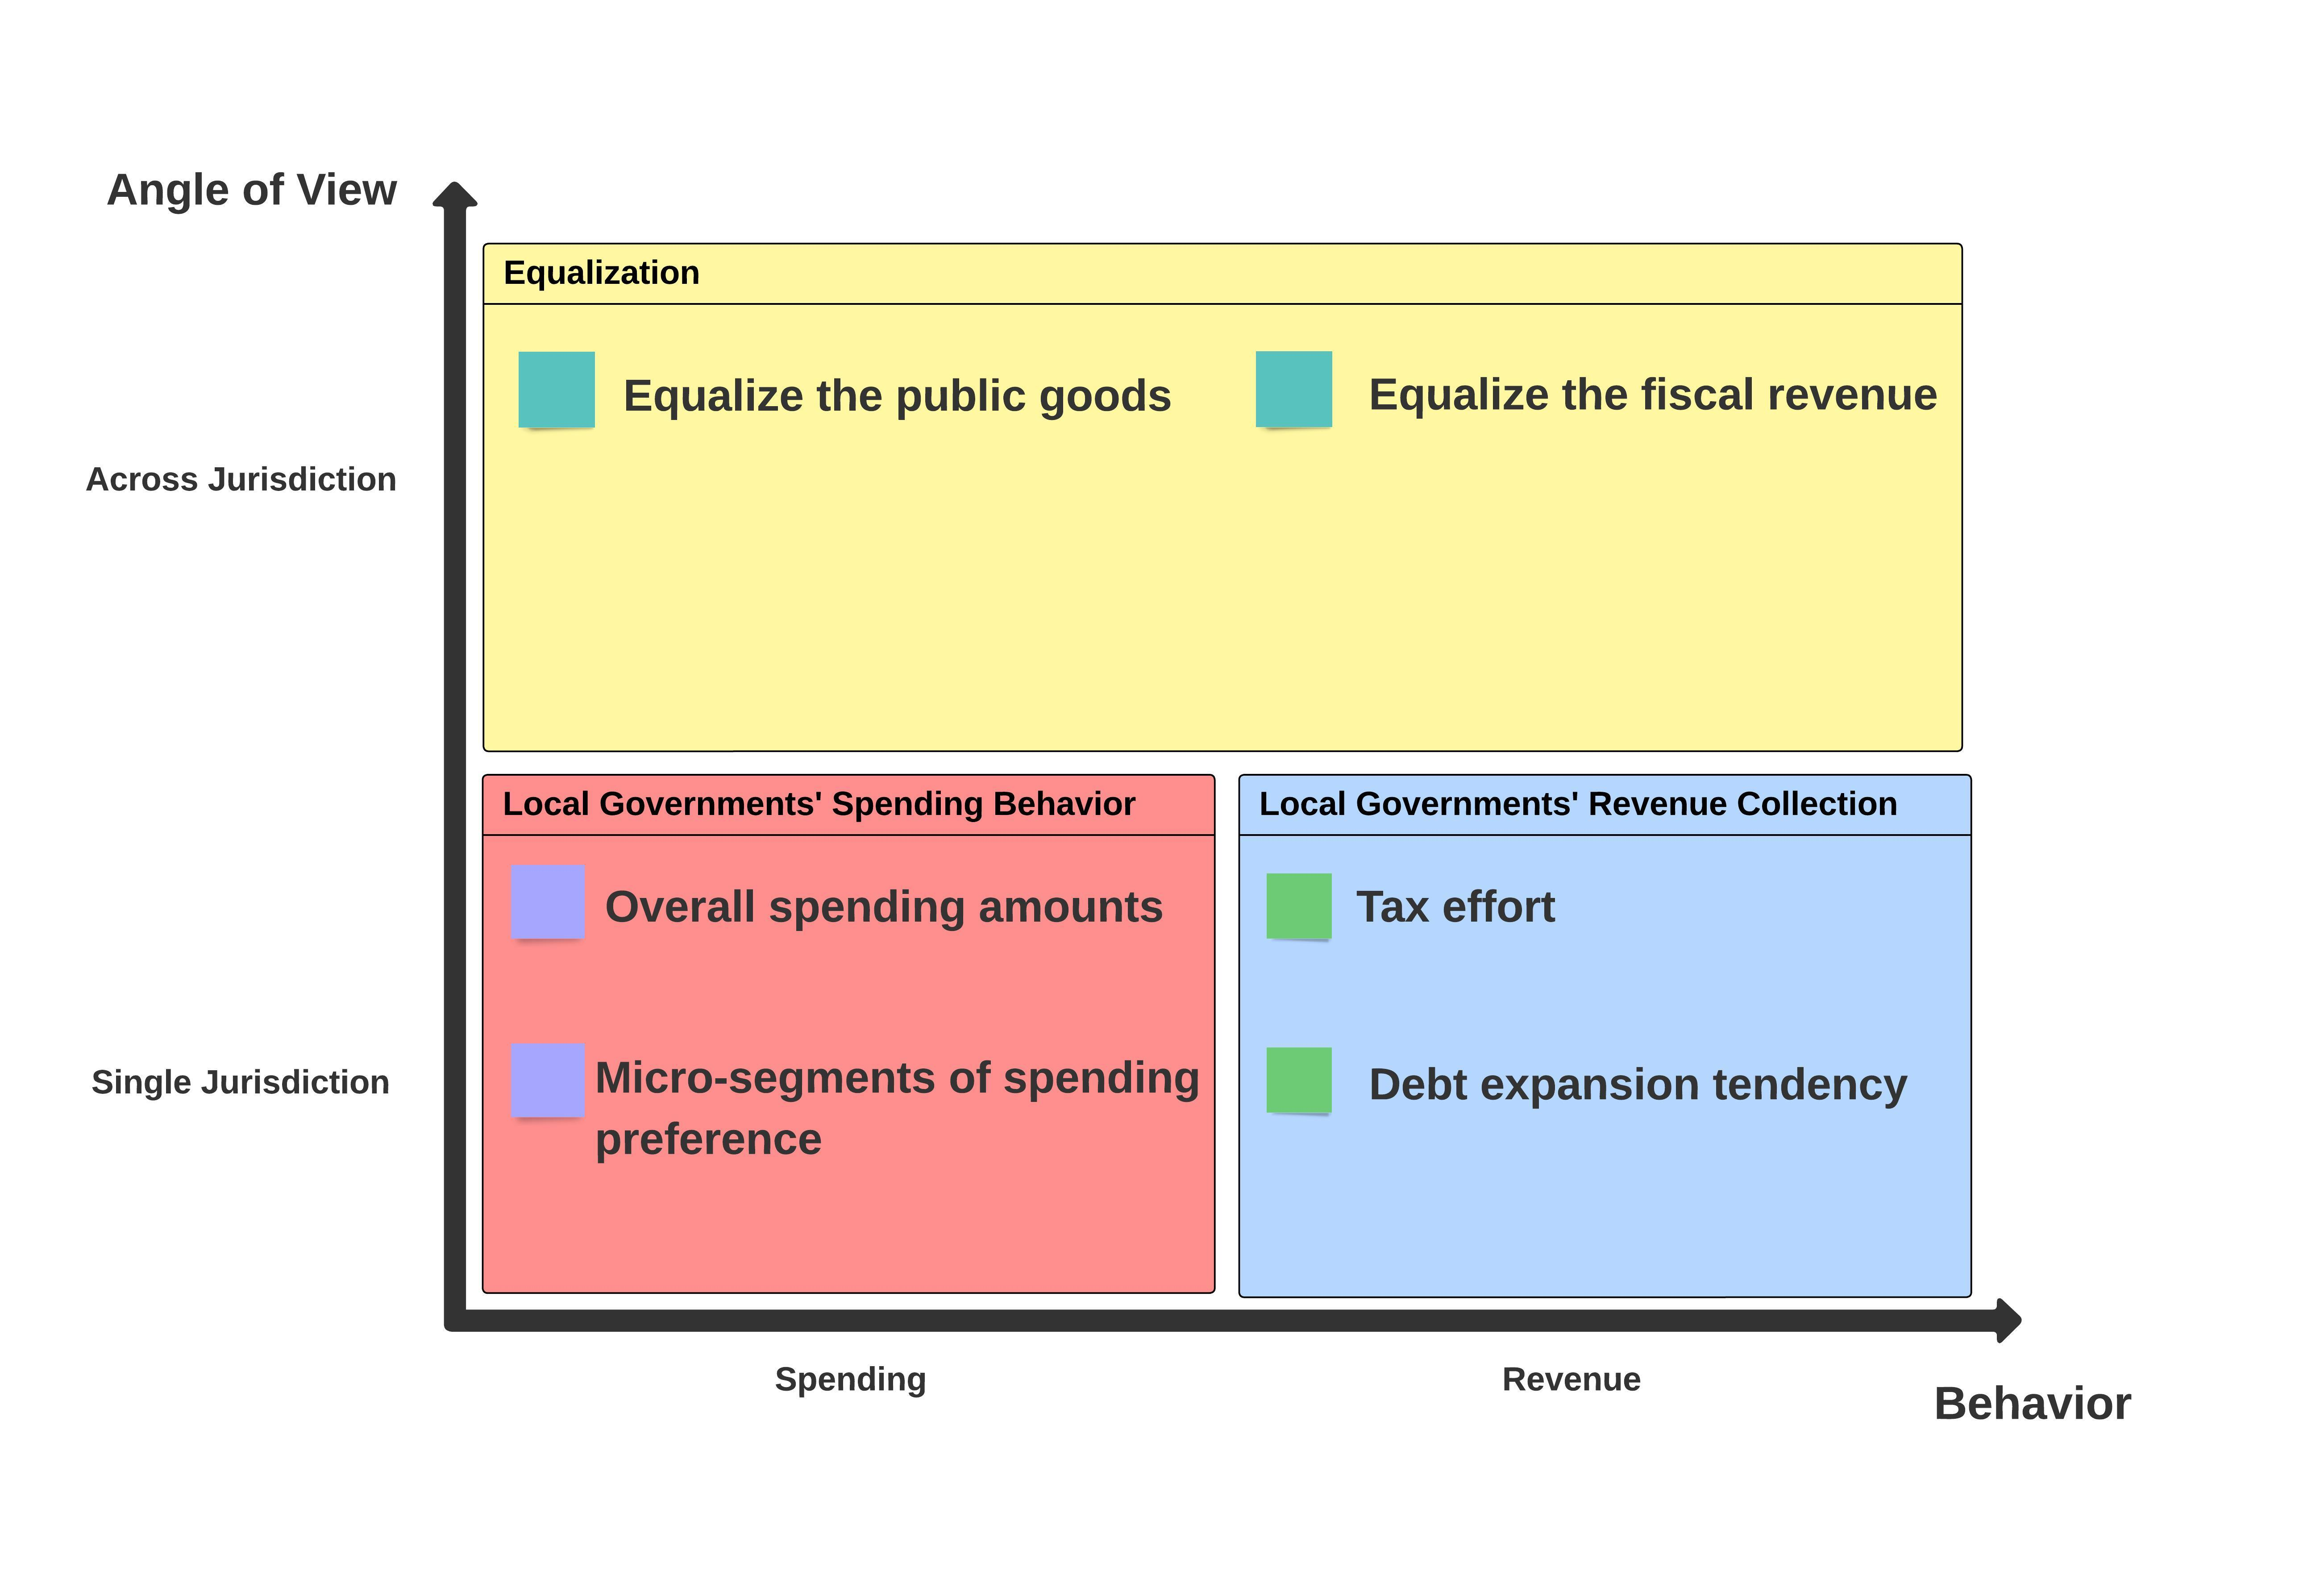
\includegraphics[scale=0.4]{Chapter-3/Figures/Effect of Intergovernmental Transfer.jpeg}
    \caption{Effect of Intergovernmental Transfer
        \texttt{} }
    \label{Figure 3.1}
\end{figure}




\section{Effect of IGT on Local Governments' Spending}

\subsection{Effect of IGT on Local Governments' Total Spending Amounts}
The most influential phenomenon during the vertical transfer from government in the fiscal federalism literature is the fly paper effect \cite{hines1995anomalies,gamkhar2007impact}. According to Bradford and Oates’s model, a lump sum grant from federal to state or local should be equivalent to the individual revenue increase within the jurisdiction in terms of the effect to stimulate the public expenditure \cite{bradford1971analysis}. The result conclusion is latterly known as equivalence theorem. Two assumptions play fundamental role in equivalence theorem. One is median voter theorem, another one is that federal, state and local government collect tax through lump sum tax. Under this theorem, money is money. However, the empirical evidence doesn’t support this theorem. More specifically, some researchers find that 1 dollar increase in personal increase would increase public expenditure by 0.02 to 0.05 dollar, while 1 dollar increase of intergovernmental transfer would trigger an increase of 0.25 to even 1 dollar in public expenditure \cite{bailey1998flypaper,dollery1996empirical,gamkhar2007impact}. This effect is known as flypaper effect. According to Inman's statistics, over 3,500 research papers investigate the flypaper effect both theoretically and empirically \cite{inman2008flypaper}.

In this section, I’m summarizing how scholars in different stages explain the flypaper effect. The understanding of flypaper effect went through a incremental progress, though may not be chronologically. This progress can be identified as three phrases. . In the first stage, the conventional analysis, scholars believe the matching grants have both price effect and income effects while the non-matching grants is analogous to the lump-sum subsidy, which means only income effects exists. In second stage, some scholars start to realize that non-matching grants has price effects as well, but that’s due to the impact of fiscal federalism setting and fiscal illusion. Federal government collecting revenue then redistributing to state and local generates fiscal illusion since this process is too complicated for consumers to perceive. In third stage, scholars start to realize the effect of distortionary tax that collect by grants recipient. The distortionary tax policy together with the low administrative efficiency in state and local leads to a higher marginal cost of the tax collection. Hence no matter the grants is matching or non-matching, the state or local government trend to use the grants rather than the tax revenue to cover the expenditure.

I set up a theoretical model and introduced the asymmetric setting into the model to explain all the local governments' reactions mentioned above. Started from a very simple Ramsey model and generalize it to more complicated scenarios.

\textbf{Benchmark model}

The Benchmark model is similar to Carlos and Guillermo's \cite{vegh2016unsticking} benchmark model with small modification.

To make the benchmark model as straight forward as possible while capture the IGT mechanism. I assume that:

\begin{enumerate}
    \item Economy is static.
    \item Only one local government and representative citizen in this economy.
    \item Two kinds of goods in the economy which are public good $G$ \label{G} and private good $X$.\label{X}
    \item Resident spend all there income $y$, which is given, on either private goods $X$ or tax $\tau$.\label{y}
    \item The tax is lump-sum tax with no dissertation.
    \item Source of government revenue: tax $\tau$ and transfer $f$.\label{f}
    \item Type of transfer: Nonmatching grants,like lump-sum subsidy.
\end{enumerate}

The representative citizen's budget constrain is:
\begin{equation}
    y=X+\tau \label{bmrc budgetc}
\end{equation}
The local government's budget constrain is:
\begin{equation}
    f+\tau=G \label{bmlg budgetc}
\end{equation}
Combine equation \ref{bmrc budgetc} and \ref{bmlg budgetc}, I get a budget constrain for the economy:
\begin{equation}
    y+f=X+G \label{bmecoconstrain}
\end{equation}
The utility for representative resident comes from the utility of $X$ and $G$. I assume the utility function is the Cobb-Douglas form thus it's a concave utility:
\begin{equation}
    U(X,G)=AX^{\alpha}G^{1-\alpha} , 0<\alpha<1 \label{bmrcutility}
\end{equation}
For the representative resident, the problem is to choose proper level of $X$ to maximize the utility in equation \ref{bmrcutility} subject to equation \ref{bmrc budgetc}. The Lagrangian equation can be set up as:
\begin{equation}
    L(X)=AX^{\alpha}G^{1-\alpha}+\lambda_{rc}(y-X-\tau)  \label{bmrclagrangian}
\end{equation}
Solving the equation \ref{bmrclagrangian} will get first order condition(foc):
\begin{equation}
    \alpha A\left(\frac{X}{G}\right)^{\alpha-1}=\lambda_{r c} \label{lamdarc}
\end{equation}
\begin{equation}
    y=X+\tau \label{rcfoc}
\end{equation}
To solve the Ramsey problem, the Ramsey planner needs to decide the level of $X,G$ to maximize the utility subject to equation \ref{bmecoconstrain} and equation \ref{bmlg budgetc}. The Lagrangian can be set as:
\begin{equation}
    L(X,G)=AX^{\alpha}G^{1-\alpha}+\lambda_{e}(y+f-X-G)+\lambda_{lg}(f+\tau-G)  \label{bmeclagrangian}
\end{equation}
Solving the equation \ref{bmeclagrangian} will generate:
\begin{equation}
    \alpha A\left(\frac{X}{G}\right)^{\alpha-1}=\lambda_e+\lambda_{l g}
    \label{foc on X}
\end{equation}
\begin{equation}
    (1- \alpha) A\left(\frac{X}{G}\right)^{\alpha}=\lambda_e+\lambda_{l g} \label{foc on G}
\end{equation}
\begin{equation}
    y+f=X+G \label{foc on lambdae}
\end{equation}
\begin{equation}
    f+\tau=G \label{foc on lambdalg}
\end{equation}

Combining equation \ref{foc on X}, \ref{foc on G}, \ref{foc on lambdae} will generate:
\begin{equation}
    (1-\alpha)y+(1-\alpha)f=G \label{bmresult}
\end{equation}
The flypaper effect definition can be mathematically expressed as $\frac{d G}{d f}-\frac{d G}{d y}$. Given equation \ref{bmresult}, the flypaper effect $fe=0$, which means, under this setting, theoretically there should be no flypaper effect.
\subsubsection{Phrase One}
Except for the introduction of intergovernmental transfer in \ref*{chapter1:Introduction}, One important concern about IGT in economic analysis is the matching mechanism. For matching grants, federal governments will reimburse a specific ratio for each 1 dollar of state and local expenditure. Based on whether federal government set a cap on the matching grants, matching grants can be divided into open-ended matching grants and closed-ended grants.

\textbf{Model with matching grants}

I loosen the last assumption in the benchmark model, now the intergovernmental transfer is 100\% matching grants which is expressed as $f_m$. Suppose the matching ratio is $m$ and $0<m<1$  \label{mr}.Thus the new budget constrain for local government is:
\begin{equation}
    \left\{\begin{array}{l} \label{mlgbudgetc}
        f_m+\tau=G \\
        f_m=m G
    \end{array}\right.
\end{equation}
And the budget constrain for the whole economy is:
\begin{equation}
    \left\{\begin{array}{l} \label{mebudgetc}
        y+f_m=X+G_M \\
        f_m=m G
    \end{array}\right.
\end{equation}
Thus the Ramsey problem is to choose proper level of $X$ and $G$ to maximize the utility subject to equation \ref{mebudgetc} and equation \ref{mlgbudgetc}.
So the new Lagrangian can be listed as:

\begin{equation} \label{mlagrangian}
    L(X,G)=AX^{\alpha}G^{1-\alpha}+\lambda_{e}(y+f_m-X-G)+\lambda_{lg}(f+\tau-G)
\end{equation}

Solving the equation \ref{mlagrangian}, I get foc conditions:
\begin{equation} \label{mfocs}
    \left\{\begin{array}{l}\alpha A \frac{X^{\alpha-1}}{G^{\alpha-1}}=\lambda_e+\lambda_{l g} \\ (1-\alpha) \frac{X^\alpha}{G^\alpha}=\lambda_e+\lambda_{l g} \\ y=X+(1-m) G\end{array}\right.
\end{equation}

By letting focs in equation \ref{mfocs} equals to zero, I get following equations:
\begin{equation} \label{myxandg}
    y=\frac{(1-\alpha)(1-m)+1}{1-\alpha} G
\end{equation}

thus the flypaper effect is calculated as $fe=\frac{d G}{d f_m}-\frac{d G}{d y}$
which equals to:
\begin{equation} \label{mfe}
    \frac{d G}{d f_m}-\frac{d G}{d y}=\frac{2 m \alpha-2 m-\alpha+2}{m[(1-\alpha)(1-m)+1]}
\end{equation}

Equation \ref{mfe} could be proved to be greater than zero, which means for matching grants, the marginal contribution on public spending is higher than the marginal contribution of private income increase.\footnote[1]{The proof process is supplied in Appendix C}

The matching grants model explains why scholars in first stage explain the fly paper effect due to misspecification or omitted variable. Misspecification means researchers may mix up matching grants with lump-sum grants. \cite{lankford1987note,henderson1968local}. Matching grants lower down the marginal price of public services, thus the mix-up will generate price effect and lead to more public goods spending \cite{gramlich1997state}. Some scholars attribute fly paper effects to omitted variables or pre-selection issue. Knight \cite{knight2002endogenous} designed a two-level bargaining model to prove that, federal government spread IGT to states and local governments with higher propensity to spend, so the flypaper effect is not a result of IGT. Former observations and investigations has endogenous issue. He also did an empirical test in which he designed an instrument variable to control the endogenous problem. He concludes that once we filter out the pre-selection issue, the flypaper effect is not obvious, at least for the data he collected about interstate highway programs. To summarize, the understanding under this view is that the flypaper effect doesn’t actually exist, it's just some kind of misspecification.

\subsubsection{Phrase two}
% In stage two, scholars start to realize that lump-sum grants also have price effect. This is a huge step since in stage one, scholars recognized the price effect of matching grants however don’t think that’s enough to explain the huge impact of flypaper effect. If non-matching grants also have price effect, then it may be enough in explaining. But in this stage, scholars claims that the price effect of non-matching grants exists because of the fiscal illusion. McCulloch (1967) argues that taxpayers misperceived  the  costs  of governmental activity, which latterly be summarized as fiscal illusions. Oates (1979), Borge (1995) first notice the price effect of non-matching grants and try to use fiscal illusion to explain the price effect. Because residents don’t recognize the actual price of the public goods. The low-estimated public good price generates a flatter slope of the budget constraint represented as l_5 in figure 7. The lower perceive leads to a greater expenditure G_2. This process reflects more clearly in figure 8. The vertical axis is not marginal substitute ration (MSR) or marginal cost of public goods as in figure 6, but a marginal cost perceived (MCP) by residents, the ratio between MCP and MSR is α=MCP/MSR. In stage one, scholars just assume α=1, which means residents fully and precisely recognize the public goods price.

% Why α≠1? Most explanation lies in the institutional setting and administrative transparency. The fiscal federalism requires federal collect the revenue and redistribute through IGT. This process is too complicated for residents to perceive. For administrative explanation, the administration process is not transparent enough for residents to understand every step. Hence, residents fail to recognize that the intergovernmental grants are collected from their income as well. Turnbull (1998) concludes in his empirical research that imperfect information generates broader fiscal illusion based on the municipal data.



\subsubsection{Phrase Three}


\subsection{Effect of IGT on Local Governments' Spending Segments}


\section{}




